\documentclass[12pt,a4paper,oneside]{article}

\usepackage[utf8]{inputenc}
\usepackage[T1]{fontenc}
\usepackage[french]{babel}
\usepackage{amssymb}
\usepackage{amsmath}
\usepackage{graphicx}


\author{Matteo Besançon}
\title {TP6 Outils formels de modélisation}
\date{\today}
\begin{document}
	\maketitle
	\setcounter{section}{1}
	\section{Dans la peau d’un apollon}
		\paragraph{Définition}

		\begin{enumerate}
			\item $C(x, y)$ : $x$ est en couple avec $y$
			\item $C(x, y) \implies C(y, x)$
			\item $A(x, y)$ : $x$ aime $y$
			\item $H = \{A_{h}, R, M\}$
			\item $F = \{A_{f}, F \}$
		\end{enumerate}

		\paragraph{On a donc :}

		\begin{enumerate}
			\item Alex est en couple avec Alex et Robin est en couple avec Floriane
				$$C(A_{h}, A_{f})$$
				$$C(R, F)$$

			\item Il y a une femme et un homme qui aiment leur partenaire respectif mais qui ont aussi des sentiments pour une autre personne

				$$\exists x \in F\ \exists y\ \exists z\ C(x, y) \wedge A(x, y) \wedge A(x, z)$$
				$$\exists x \in H\ \exists y\ \exists z\ C(x, y) \wedge A(x, y) \wedge A(x, z)$$

			\item Il y a une femme et un homme qui n’aiment que leur partenaire respectif

				$$\exists x \in F\ \exists y\ \forall  z\neq y\ C(x, y) \wedge A(x, y) \wedge \neg A(x, z)$$
				$$\exists x \in H\ \exists y\ \forall z\neq y\ C(x, y) \wedge A(x, y) \wedge \neg A(x, z)$$

			\item Miguel commence à éprouver des sentiments pour une personne qui aime une personne qui aime Alexandrine

				$$\exists x\ \exists y\ A(M, x) \wedge A(x, y) \wedge A(y, A_{f})$$

			\item Toutes les femmes n’aiment que des hommes

				$$\forall x \in F\ \exists y \in F\ \neg A(x, y)$$

			\item Robin aime une personne dans un triangle amoureux

				$$\exists x\ \exists y\ A(R, x) \wedge A(x,y) \wedge A(y, R)$$

			\item Personne ne s’aime soi-même

				$$\exists x\ \neg A(x, x)$$

		\end{enumerate}

		\begin{figure}[h]
			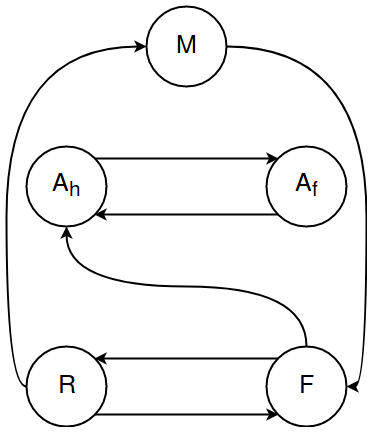
\includegraphics[scale = 0.7]{ex1.png}
			\centering
			\caption{Graphe des relations amoureuses}
			\label{lab1}
		\end{figure}

		\section{Saison 2}

		On cherche à prouver soit il y a une relation incestueuse, soit Miguel n’est pas
		amoureux de Floriane.

		Or nous avons à la figure \ref{lab1} un contre exemple nous permettant de prouver que
		c'est faux. En effet dans notre cas que Miguel ou Robin soit le frère de Alex il n'y a
		pas de relation incestueuse. Et qui plus est Miguel est amoureux de Floriane.

		Notre amis a donc raison.

\end{document}
